
\paragraph{UC-46 Creazione di una nuova prenotazione}
    \begin{itemize}
	    \item \textbf{Attore primario:} dipendente;

	    \item \textbf{Descrizione:} il dipendente vuole effettuare una prenotazione. La prenotazione è identificata da un codice univoco, una data, un orario, una stanza e una postazione;

	    \item \textbf{Precondizioni:} il dipendente ha selezionato la funzionalità di creazione di una nuova prenotazione;

	    \item \textbf{Postcondizioni:} il dipendente ha creato una prenotazione;

	    \item \textbf{Scenario principale:}
	        \begin{enumerate}
		        \item il dipendente seleziona una stanza da una lista di stanze disponibili (UC-46.1 Selezione stanza);
		        \item il dipendente seleziona una postazione da una lista di postazioni disponibili all'interno della stanza (UC-46.2 Selezione stanza); 
		        \item il dipendente seleziona la data in cui effettuare la prenotazione (UC-46.3 Seleziona data);
		        \item il dipendente seleziona l'orario in cui intende far partire la prenotazione della postazione (UC-46.4 Selezione orario d'inizio);
		        \item il dipendente seleziona la durata della propria prenotazione (UC-46.5 Selezione della durata);
	        \end{enumerate}
    \end{itemize}

    \begin{figure}[H]
		\centering
		  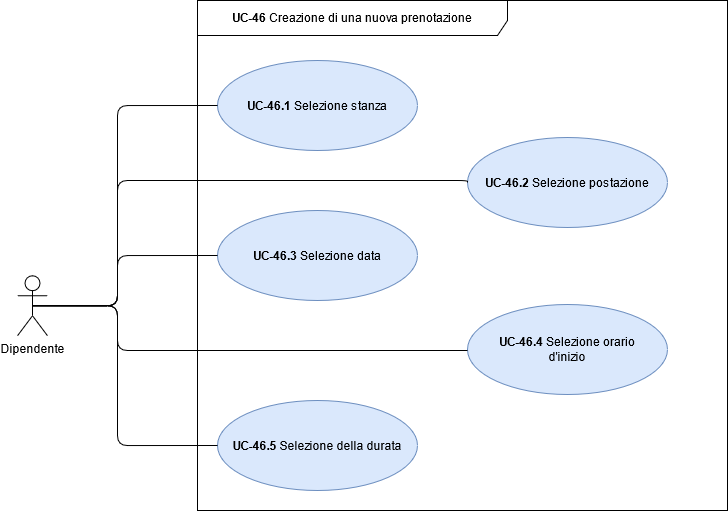
\includegraphics[scale=0.50]{src/CasiDUso/immagini/CreazionePrenotazione.png}
		\caption{Diagramma relativo alla creazione di una nuova prenotazione da applicazione mobile}
	\end{figure}

\paragraph{UC-46.1 Selezione stanza}

    \begin{itemize}
	    \item \textbf{Attore primario:} dipendente;

	    \item \textbf{Descrizione:} il dipendente vuole selezionare la stanza nella quale prenotare una postazione da una lista di stanze disponibili (non piene o disabilitate);

	    \item \textbf{Precondizioni:} il dipendente ha selezionato il form in cui inserire la stanza ricercata;

	    \item \textbf{Postcondizioni:} il dipendente ha inserito con successo la stanza in cui è presente la postazione che vuole prenotare;

	    \item \textbf{Scenario principale:}
	        \begin{enumerate}
		        \item il dipendente seleziona una stanza da una lista di stanze disponibili nel form;
	        \end{enumerate}
    \end{itemize}

\paragraph{UC-46.2 Selezione postazione}

    \begin{itemize}
        \item \textbf{Attore primario:} dipendente;

        \item \textbf{Descrizione:} il dipendente vuole selezionare la postazione da prenotare all'interno della stanza da una lista di postazioni prenotabili (le postazioni in questione non possono essere occupate o disabilitate);

        \item \textbf{Precondizioni:} il dipendente ha selezionato il form in cui inserire la postazione da prenotare;

        \item \textbf{Postcondizioni:} il dipendente ha inserito con successo la postazione da prenotare;

        \item \textbf{Scenario principale:}
            \begin{enumerate}
                \item il dipendente seleziona una postazione dalla lista di postazioni prenotabili  nella stanza;
            \end{enumerate}
    \end{itemize}

\paragraph{UC-46.3 Selezione data}

    \begin{itemize}
        \item \textbf{Attore primario:} dipendente;

        \item \textbf{Descrizione:} il dipendente vuole selezionare la data di prenotazione della postazione scelta da un elenco di date disponibili;

        \item \textbf{Precondizioni:} il dipendente ha selezionato il form in cui inserire la data di prenotazione;

        \item \textbf{Postcondizioni:} il dipendente ha inserito con successo la data di prenotazione;

        \item \textbf{Scenario principale:}
            \begin{enumerate}
                \item il dipendente seleziona una data dall'elenco di date disponibili;
            \end{enumerate}
    \end{itemize}


\paragraph{UC-46.4 Selezione orario d'inizio}

    \begin{itemize}
        \item \textbf{Attore primario:} dipendente;

        \item \textbf{Descrizione:} il dipendente vuole selezionare l'orario d'inizio della postazione;

        \item \textbf{Precondizioni:} il dipendente ha selezionato il form in cui inserire l'orario d'inizio della prenotazione;

        \item \textbf{Postcondizioni:} il dipendente ha inserito con successo l'orario d'inizio della prenotazione;

        \item \textbf{Scenario principale:}
            \begin{enumerate}
                \item il dipendente seleziona un orario disponibile da una lista di orari in cui la prenotazione è prenotabile;
            \end{enumerate}
    \end{itemize}

\paragraph{UC-46.5 Selezione della durata}

    \begin{itemize}
        \item \textbf{Attore primario:} dipendente;

        \item \textbf{Descrizione:} il dipendente vuole selezionare la durata della propria prenotazione (in intervalli da 30 minuti);

        \item \textbf{Precondizioni:} il dipendente ha selezionato il form in cui inserire l'intervallo di tempo di utilizzo della postazione;

        \item \textbf{Postcondizioni:} il dipendente ha inserito con successo la durata della propria prenotazione;

        \item \textbf{Scenario principale:}
            \begin{enumerate}
                \item il dipendente seleziona la durata della propria prenotazione da un elenco di intervalli di tempo;
            \end{enumerate}
    \end{itemize}
  
\paragraph{UC-47 Visualizzazione delle prenotazioni effettuate}

    \begin{itemize}
        \item \textbf{Attore primario:} dipendente;

        \item \textbf{Descrizione:} il dipendente vuole visualizzare lo storico delle proprie prenotazioni;

        \item \textbf{Precondizioni:} il dipendente ha selezionato la funzionalità di visualizzazione delle proprie prenotazioni;

        \item \textbf{Postcondizioni:} il dipendente può visualizzare tutte le prenotazioni da lui effettuate;

        \item \textbf{Scenario principale:}
            \begin{enumerate}
                 \item il sistema restituisce un elenco contenente tutte le prenotazioni effettuate da un dipendente. Il dipendente può visualizzare l'ID (UC-47.1 Visualizzazione id prenotazione), la data (UC-47.2 Visualizzazione data), l'ora di inizio (UC-47.3 Visualizzazione orario d'inizio), la stanza (UC-47.4 Visualizzazione stanza), il codice della postazione prenotata (UC-47.5 Visualizzazione codice postazione) e la durata (UC-47.6 Visualizzazione della durata della prenotazione) a partire da una singola prenotazione;
            \end{enumerate}
    \end{itemize}

    \begin{figure}[H]
		\centering
		  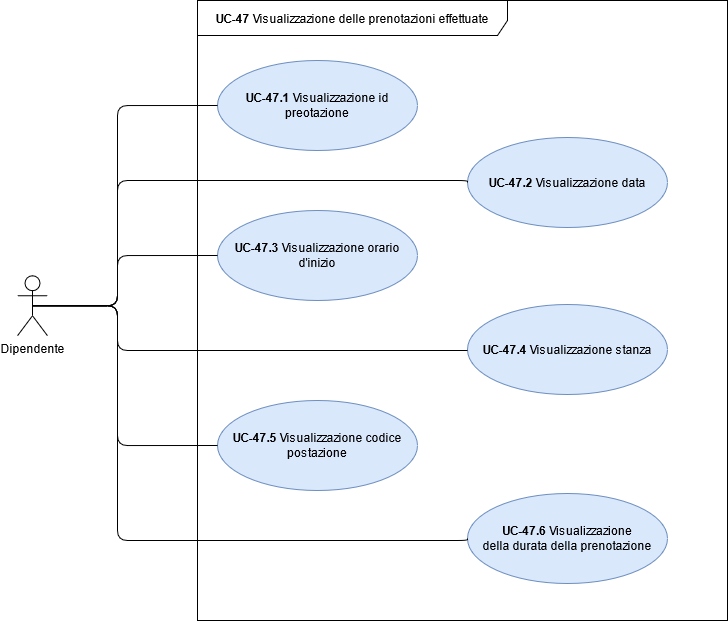
\includegraphics[scale=0.40]{src/CasiDUso/immagini/VisualizzazionePrenotazioni.png}
		\caption{Diagramma relativo alla visualizzazione delle prenotazioni effettuate da mobile}
	\end{figure}


\paragraph{UC-47.1 Visualizzazione id prenotazione}
    
    \begin{itemize}
        \item \textbf{Attore primario:} dipendente;

        \item \textbf{Descrizione:} il dipendente vuole visualizzare l'id di una specifica prenotazione;

        \item \textbf{Precondizioni:} il dipendente ha selezionato la prenotazione da visualizzare in dettaglio;

        \item \textbf{Postcondizioni:} il dipendente può visualizzare l'id della prenotazione selezionata;

        \item \textbf{Scenario principale:}
            \begin{enumerate}
                 \item il sistema aggiorna la schermata mostrando a video le informazioni in dettaglio (tra cui l'ID) relative alla prenotazione selezionata.
            \end{enumerate}
    \end{itemize}

\paragraph{UC-47.2 Visualizzazione data}

    \begin{itemize}
        \item \textbf{Attore primario:} dipendente;

        \item \textbf{Descrizione:} il dipendente vuole visualizzare la data di una specifica prenotazione;

        \item \textbf{Precondizioni:} il dipendente ha selezionato la prenotazione da visualizzare in dettaglio;

        \item \textbf{Postcondizioni:} il dipendente può visualizzare la data della prenotazione selezionata;

        \item \textbf{Scenario principale:}
            \begin{enumerate}
                 \item il sistema aggiorna la schermata mostrando a video le informazioni in dettaglio (tra cui la data) relative alla prenotazione selezionata.
            \end{enumerate}
    \end{itemize} 

\paragraph{UC-47.3 Visualizzazione orario d'inizio}

    \begin{itemize}
        \item \textbf{Attore primario:} dipendente;

        \item \textbf{Descrizione:} il dipendente vuole visualizzare l'orario d'inizio di una specifica prenotazione;

        \item \textbf{Precondizioni:} il dipendente ha selezionato la prenotazione da visualizzare in dettaglio;

        \item \textbf{Postcondizioni:} il dipendente può visualizzare l'orario d'inizio della prenotazione selezionata;

        \item \textbf{Scenario principale:}
            \begin{enumerate}
                 \item il sistema aggiorna la schermata mostrando a video le informazioni in dettaglio (tra cui l'orario d'inizio) relative alla prenotazione selezionata.
            \end{enumerate}
    \end{itemize} 

\paragraph{UC-47.4 Visualizzazione stanza}

    \begin{itemize}
        \item \textbf{Attore primario:} dipendente;

        \item \textbf{Descrizione:} il dipendente vuole visualizzare la stanza di una specifica prenotazione;

        \item \textbf{Precondizioni:} il dipendente ha selezionato la prenotazione da visualizzare in dettaglio;

        \item \textbf{Postcondizioni:} il dipendente può visualizzare la stanza della prenotazione selezionata;

        \item \textbf{Scenario principale:}
            \begin{enumerate}
                 \item il sistema aggiorna la schermata mostrando a video le informazioni in dettaglio (tra cui la stanza) relative alla prenotazione selezionata.
            \end{enumerate}
    \end{itemize} 

\paragraph{UC-47.5 Visualizzazione codice postazione}

    \begin{itemize}
        \item \textbf{Attore primario:} dipendente;

        \item \textbf{Descrizione:} il dipendente vuole visualizzare il codice della postazione prenotata in una specifica prenotazione;

        \item \textbf{Precondizioni:} il dipendente ha selezionato la prenotazione da visualizzare in dettaglio;

        \item \textbf{Postcondizioni:} il dipendente può visualizzare il codice della postazione della prenotazione selezionata;

        \item \textbf{Scenario principale:}
            \begin{enumerate}
                \item il sistema aggiorna la schermata mostrando a video le informazioni in dettaglio (tra cui il codice della postazione prenotata) relative alla prenotazione selezionata.
            \end{enumerate}
    \end{itemize} 

\paragraph{UC-47.6 Visualizzazione della durata della prenotazione}

    \begin{itemize}
        \item \textbf{Attore primario:} dipendente;

        \item \textbf{Descrizione:} il dipendente vuole visualizzare la durata di una specifica prenotazione;

        \item \textbf{Precondizioni:} il dipendente ha selezionato la prenotazione da visualizzare in dettaglio;

        \item \textbf{Postcondizioni:} il dipendente può visualizzare la durata della prenotazione selezionata;

        \item \textbf{Scenario principale:}
            \begin{enumerate}
                \item il sistema aggiorna la schermata mostrando a video le informazioni in dettaglio (tra cui la durata) relative alla prenotazione selezionata.
            \end{enumerate}
    \end{itemize} 


\paragraph{UC-48 Cancellazione di una prenotazione}

    \begin{itemize}
        \item \textbf{Attore primario:} dipendente;

        \item \textbf{Descrizione:} il dipendente vuole eliminare una prenotazione futura. Le prenotazioni di postazioni già concluse non possono essere rimosse;

        \item \textbf{Precondizioni:} il dipendente ha selezionato la prenotazione da visualizzare in dettaglio;

        \item \textbf{Postcondizioni:} il dipendente ha eliminato con successo la prenotazione;

        \item \textbf{Scenario principale:}
            \begin{enumerate}
                \item il dipendente seleziona la funzionalità di cancellazione della prenotazione;
                \item il sistema aggiorna l'elenco delle prenotazioni rimuovendo quella selezionata.
            \end{enumerate}
    \end{itemize} 

\paragraph{UC-49 Marcatura postazione come igienizzata}
    \begin{itemize}
        \item \textbf{Attore primario:} dipendente;

        \item \textbf{Descrizione:} il dipendente vuole marcare una postazione come igienizzata dopo averla pulita. Per far ciò è necessario scansionare il tag RFID;

        \item \textbf{Precondizioni:} il dipendente ha selezionato la funzionalità di igienizzazione di una postazione. Il dipendente ha igienizzato la postazione;

        \item \textbf{Postcondizioni:} il dipendente ha marcato con successo la postazione come igienizzata;

        \item \textbf{Scenario principale:}
            \begin{enumerate}
                \item il dipendente seleziona la postazione da pulire da un elenco di postazioni sporche;
                \item il dipendente scansiona il tag RFID della postazione per segnalare l'avvenuta igienizzazione (UC-49.1 Scansione del tag RFID per segnalare l'avvenuta igienizzazione);
                \item il sistema aggiorna lo stato della postazione da sporca a pulita.
            \end{enumerate}
    \end{itemize} 

    \begin{figure}[H]
		\centering
		  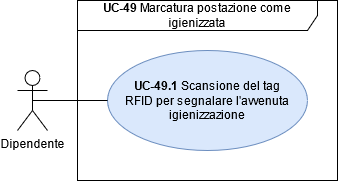
\includegraphics[scale=0.50]{src/CasiDUso/immagini/IgienizzazioneDipendente.png}
		\caption{Diagramma relativo all'igienizzazione di una postazione da parte di un dipendente}
	\end{figure}

\paragraph{UC-49.1 Scansione del tag RFID per segnalare l'avvenuta igienizzazione}
    
    \begin{itemize}
        \item \textbf{Attore primario:} dipendente;

        \item \textbf{Descrizione:} il dipendente vuole scansionare il tag RFID per segnalare l'avvenuta igienizzazione della postazione;

        \item \textbf{Precondizioni:} il dipendente ha selezionato la postazione da igienizzare;

        \item \textbf{Postcondizioni:} il dipendente ha scansionato con successo il tag RFID;

        \item \textbf{Scenario principale:}
            \begin{enumerate}
                \item il dipendente appoggia il proprio dispositivo sul tag RFID;
                \item il tag viene scansionato dall'applicazione.
            \end{enumerate}
    \end{itemize} 

\paragraph{UC-50 Scansione presenza}

    \begin{itemize}
        \item \textbf{Attore primario:} dipendente;

        \item \textbf{Descrizione:} il dipendente vuole segnalare la propria presenza su una postazione libera scansionando il tag RFID;

        \item \textbf{Precondizioni:} il dipendente ha selezionato la funzionalità di rilevamento della presenza su una postazione;

        \item \textbf{Postcondizioni:} il dipendente ha comunicato con successo la propria presenza;

        \item \textbf{Scenario principale:}
            \begin{enumerate}
                \item il dipendente seleziona la funzionalità di rilevamento della presenza;
                \item il dipendente scansiona il tag RFID della postazione in cui è seduto (UC-50.1 Scansione del tag RFID per segnalare la propria presenza nella postazione);
                \item il sistema fornisce informazioni relative allo stato della postazione (UC-50.2 Visualizzazione stato della postazione). Qualora la postazione risulti non disabilitata o non occupata il sistema invierà una richiesta di avvio dell'utilizzo;
                \item il dipendente conferma l'utilizzo della postazione (UC-50.3 Avvio utilizzo);
                \item il sistema aggiorna lo stato della postazione da libera a occupata.
            \end{enumerate}
    \end{itemize} 

    \begin{figure}[H]
		\centering
		  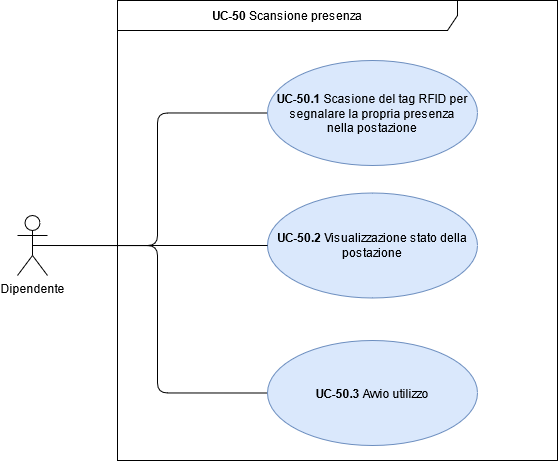
\includegraphics[scale=0.50]{src/CasiDUso/immagini/ScansionePresenza.png}
		\caption{Diagramma relativo alla segnalazione della propria presenza su una postazione}
	\end{figure}


\paragraph{UC-50.1 Scansione del tag RFID per segnalare la propria presenza nella postazione}
   
    \begin{itemize}
        \item \textbf{Attore primario:} dipendente;

        \item \textbf{Descrizione:} il dipendente vuole scansionare il tag RFID per visualizzare lo stato della postazione;

        \item \textbf{Precondizioni:} il dipendente ha selezionato la postazione da analizzare;

        \item \textbf{Postcondizioni:} il dipendente ha scansionato con successo il tag RFID;

        \item \textbf{Scenario principale:}
            \begin{enumerate}
                \item il dipendente appoggia il proprio dispositivo sul tag RFID;
                \item il tag viene scansionato dall'applicazione.
            \end{enumerate}
    \end{itemize}

\paragraph{UC-50.2 Visualizzazione stato della postazione}

\begin{itemize}
    \item \textbf{Attore primario:} dipendente;

    \item \textbf{Descrizione:} il dipendente vuole visualizzare lo stato della postazione in cui si trova;

    \item \textbf{Precondizioni:} il dipendente ha scansionato il tag RFID della postazione;

    \item \textbf{Postcondizioni:} il dipendente può visualizzare lo stato della postazione;

    \item \textbf{Scenario principale:}
        \begin{enumerate}
            \item il sistema fornisce al dipendente lo stato attuale della postazione. La postazione può essere libera/occupata, pulita/sporca o disabilitata.
        \end{enumerate}
\end{itemize}

\paragraph{UC-50.3 Avvio utilizzo}

    \begin{itemize}
        \item \textbf{Attore primario:} dipendente;

        \item \textbf{Descrizione:} il dipendente vuole confermare la volontà di utilizzo della postazione;

        \item \textbf{Precondizioni:} il dipendente ha scansionato il tag RFID della postazione. La postazione risulta libera;

        \item \textbf{Postcondizioni:} il dipendente ha confermato la volontà di utilizzare la postazione;

        \item \textbf{Scenario principale:}
            \begin{enumerate}
                \item il sistema invia al dipendente una richiesta di conferma dell'utilizzo della postazione;
                \item il dipendente conferma l'utilizzo della postazione.
            \end{enumerate}
    \end{itemize}

\paragraph{UC-51 Terminazione utilizzo della postazione}

    \begin{itemize}
        \item \textbf{Attore primario:} dipendente;

        \item \textbf{Descrizione:} il dipendente vuole terminare l'utilizzo della postazione;

        \item \textbf{Precondizioni:} il dipendente ha selezionato la prenotazione da terminare;

        \item \textbf{Postcondizioni:} il dipendente ha segnalato con successo il termine dell'utilizzo della postazione;

        \item \textbf{Scenario principale:}
            \begin{enumerate}
                \item il dipendente seleziona la funzionalità di termine della prenotazione dalla schermata della prenotazione in dettaglio;
                \item il dipendente appoggia il proprio dispositivo sul tag RFID;
                \item il tag viene scansionato dall'applicazione;
                \item il sistema elabora la richiesta, termina la prenotazione effettuata dal dipendente e marca la postazione come libera e sporca.
            \end{enumerate}
    \end{itemize} 

